A continuación se analizan los tiempos de ejecución y el consumo de memoria de los algoritmos implementados, contrastando su rendimiento empírico con su complejidad asintótica teórica. Para establecer una base comparativa clara, el Cuadro \ref{tab:teoria} resume la complejidades esperadas para cada algoritmo.

\begin{table}[htbp]
    \centering
    \caption{Complejidad teórica de los algoritmos evaluados.}
    \label{tab:teoria}
    \renewcommand{\arraystretch}{1.2}
    \begin{tabular}{|l|c|c|c|c|c|c|}
        \hline
        \textbf{Algoritmo} & \textbf{Mejor} & \textbf{Promedio} & \textbf{Peor} & \textbf{Memoria} & \textbf{Estable} & \textbf{In-place} \\
        \hline
        \texttt{std::sort} & $\mathcal{O}(N \log N)$ & $\mathcal{O}(N \log N)$ & $\mathcal{O}(N \log N)$ & $\mathcal{O}(\log N)$ & No & Sí \\
        MergeSort & $\mathcal{O}(N \log N)$ & $\mathcal{O}(N \log N)$ & $\mathcal{O}(N \log N)$ & $\mathcal{O}(N)$ & Sí & No \\
        PatienceSort & $\mathcal{O}(N)$ & $\mathcal{O}(N \log N)$ & $\mathcal{O}(N \log N)$ & $\mathcal{O}(N)$ & No & No \\
        QuickSort & $\mathcal{O}(N \log N)$ & $\mathcal{O}(N \log N)$ & $\mathcal{O}(N^2)$ & $\mathcal{O}(\log N)$ & No & Sí \\
        \hline
        Naive MatMul & $\mathcal{O}(N^3)$ & $\mathcal{O}(N^3)$ & $\mathcal{O}(N^3)$ & $\mathcal{O}(N^2)$ & N/A & No \\
        Strassen & $\mathcal{O}(N^{\log_2 7})$ & $\mathcal{O}(N^{\log_2 7})$ & $\mathcal{O}(N^{\log_2 7})$ & $\mathcal{O}(N^2)$ & N/A & No \\
        \hline
    \end{tabular}
\end{table}

\subsection{Problema de Ordenamiento}

\begin{figure}[!htbp]
    \centering
    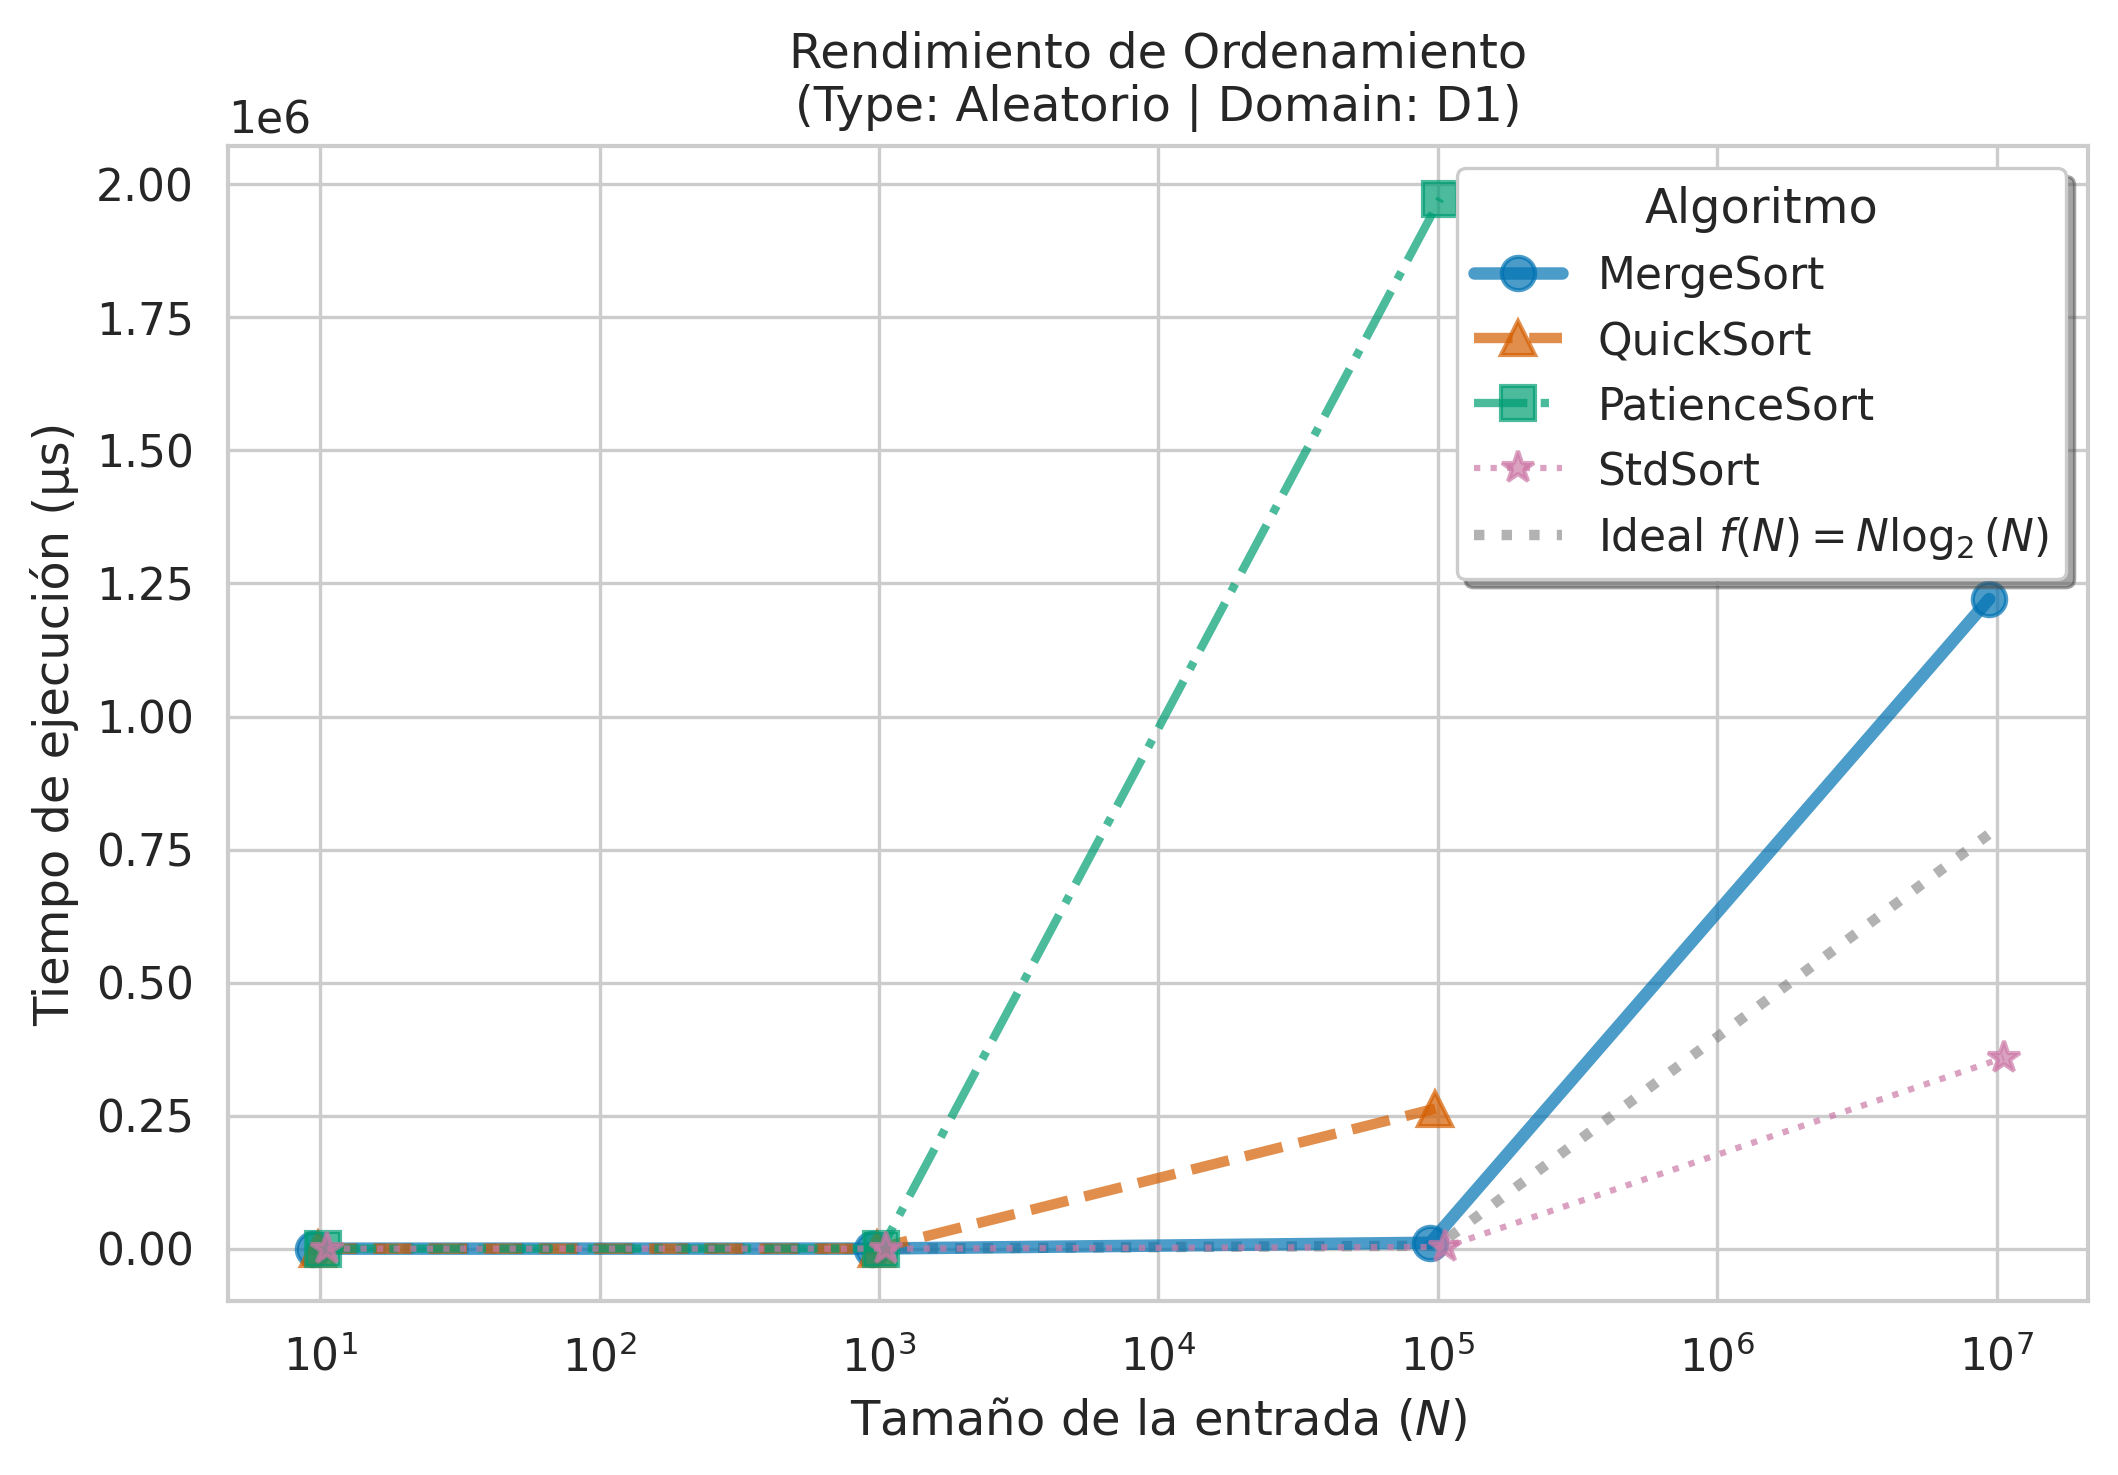
\includegraphics[width=0.7\textwidth]{../code/sorting/data/plots/sorting_time_us_aleatorio_D1.png}
    \caption{Tiempo de ejecución para arreglos aleatorios (Dominio D1).}
    \label{fig:sort_aleatorio}
\end{figure}

\textbf{Comportamiento en el caso promedio}

Para arreglos aleatorios (Figura \ref{fig:sort_aleatorio}), los algoritmos cumplen con la teoría esperada de $\mathcal{O}(N \log N)$ (Para evidenciar se trazo una línea de tendencia ideal $N \log N$ sobre el gráfico). Sin embargo, los tiempos de ejecución difieren sustancialmente: para $N=10^5$, MergeSort resuelve el problema en unos $11.000\ \mu s$ promedio, siendo notablemente más rápido que QuickSort, el cual supera los $258.000\ \mu s$. 

Esta diferencia no se explica por la complejidad teórica, sino por cómo la implementación interactúa con la memoria del computador. La implementación de QuickSort selecciona el último elemento como pivote y recorre el arreglo ejecutando incesantemente la instrucción \texttt{swap()} cada vez que encuentra un valor menor. En un arreglo desordenado, esto obliga al procesador hacer miles de sobreescrituras en memoria, frenando el rendimiento. Por otro lado, en MergeSort se gasta memoria dinámica creando subvectores temporales, su proceso de fusión avanza de manera lineal, lo que para el hardware moderno es mas llevadero. 

\textbf{Cuello de botella en Patience Sort}

En arreglos aleatorios, Patience Sort se posiciona como el algoritmo más lento \cite{aldous1999longest}, tardando entre $1.900.000\ \mu s$ y $2.000.000\ \mu s$ para $N=10^5$ (Dominio D1). Este bajo rendimiento, es resultado directo de 2 decisiones costosas en el código que castigan la memoria del computador. Durante la fase unir pilas (\texttt{merge\_piles}) el código busca el menor número iterando por todas ellas. En un arreglo aleatorio se generan muchas pilas, lo que significa un gran gasto de tiempo comparando numero por numero repetitivamente. La segunda decisión o causa dentro del código es la instrucción \texttt{v.erase(v.begin() + index)}. Borrar un elemento en medio de un vector obliga a tomar todos los elementos que están a la derecha y desplazarlos hacia la izquierda, dicho reordenamiento masivo miles de veces hace que se disparen los tiempos de ejecución. 

\begin{figure}[!htbp]
    \centering
    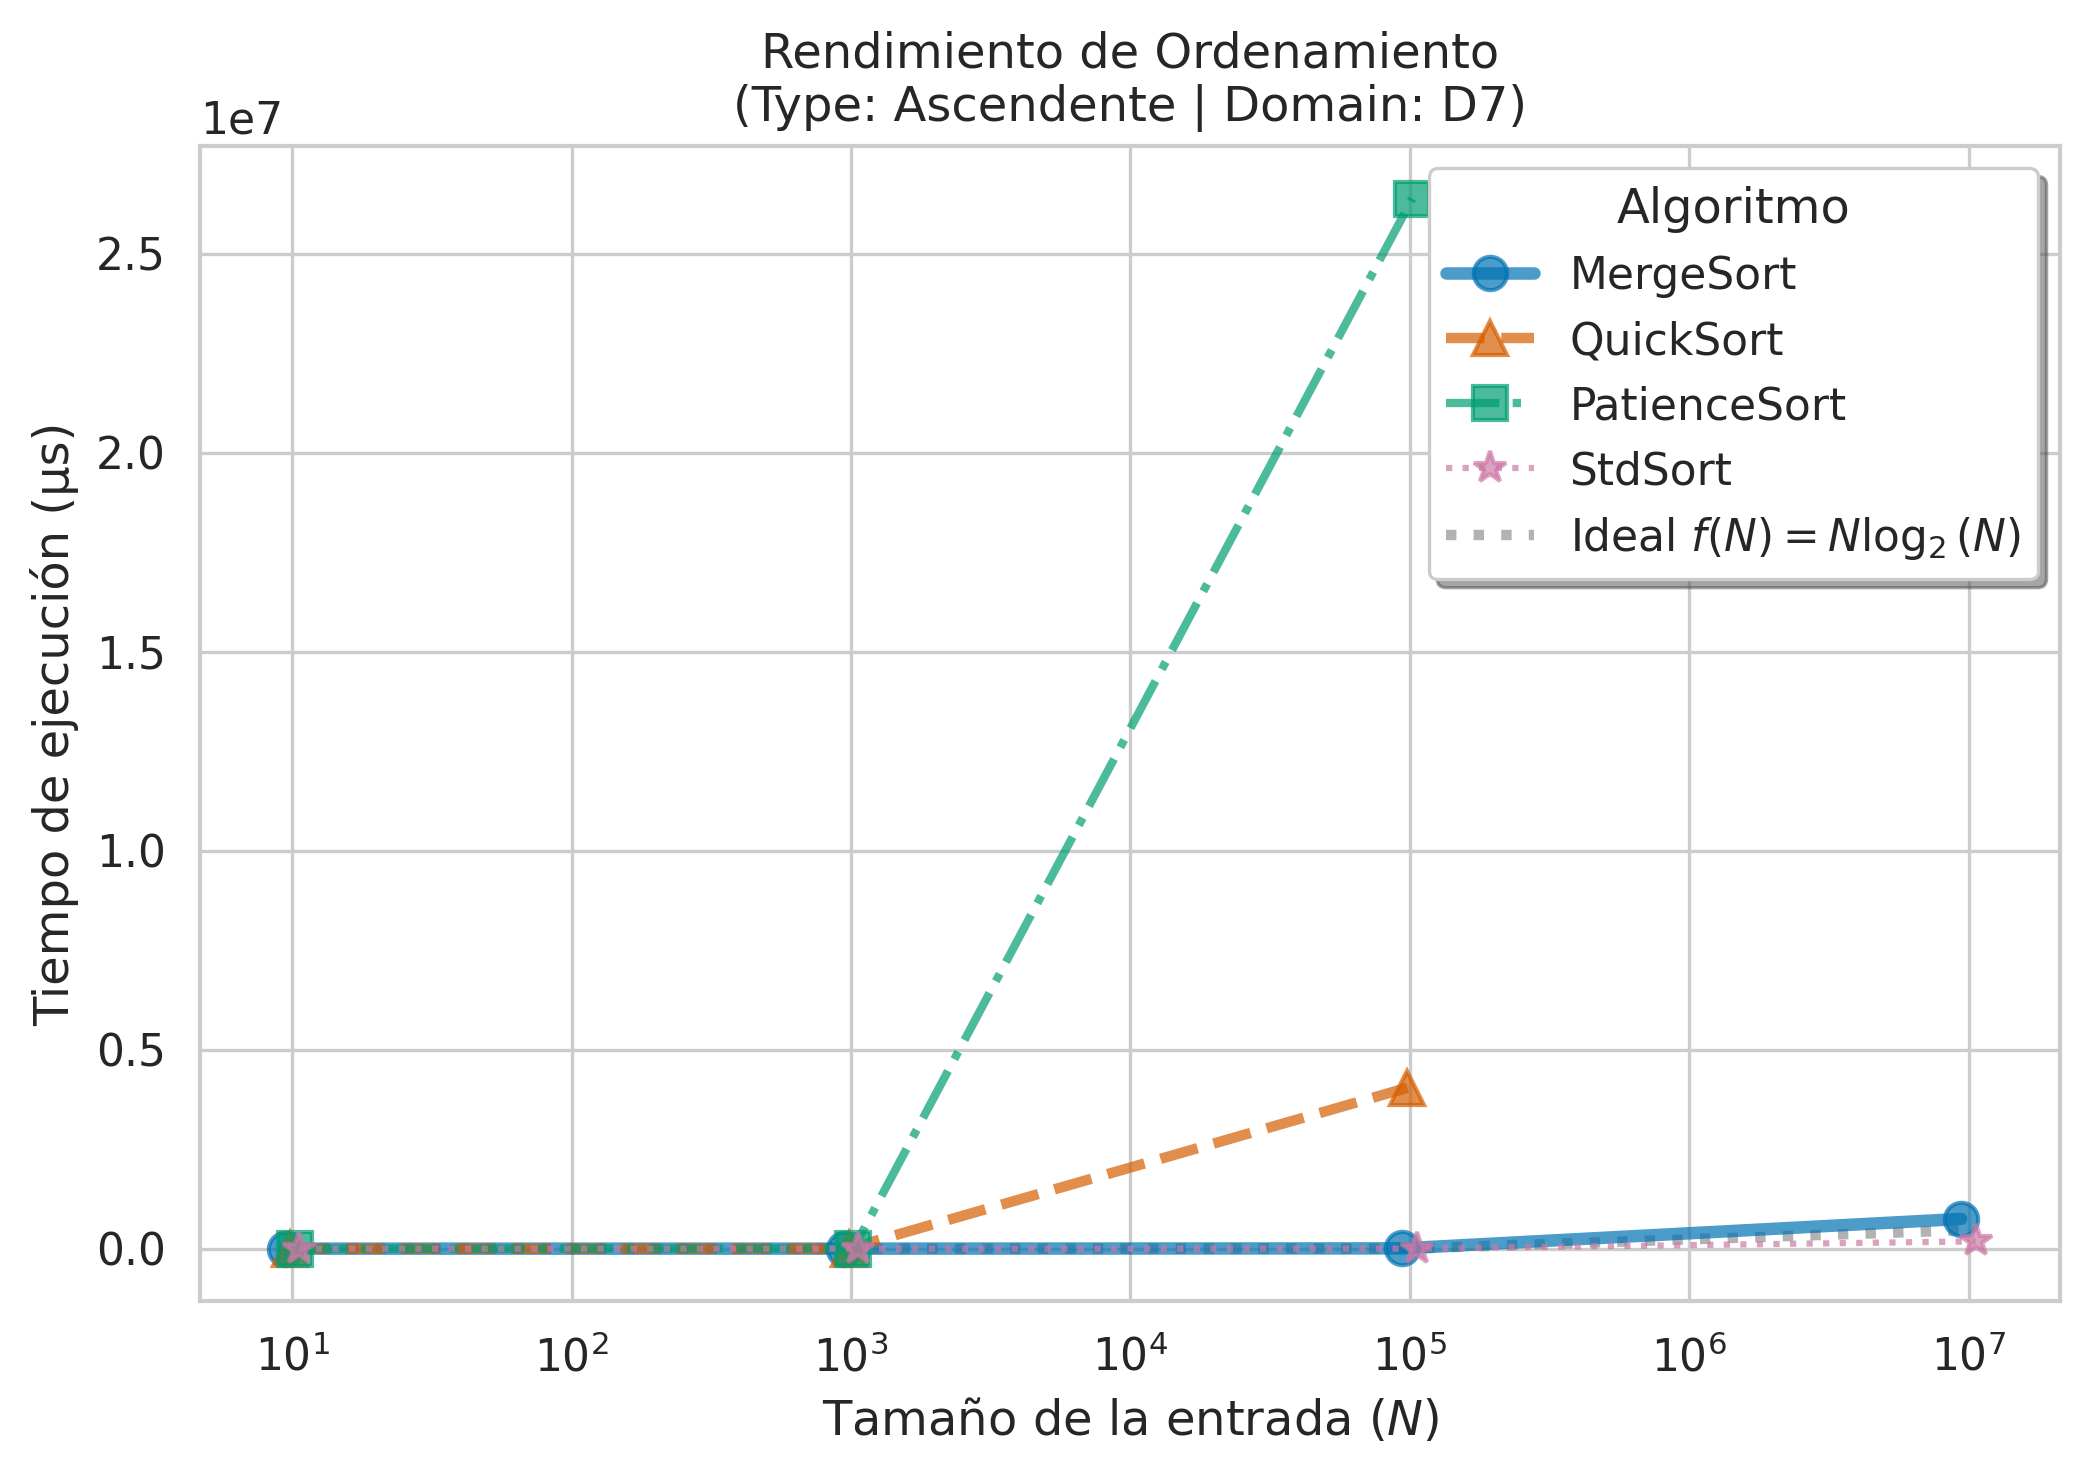
\includegraphics[width=0.7\textwidth]{../code/sorting/data/plots/sorting_time_us_ascendente_D7.png}
    \caption{Tiempo de ejecución para arreglos ascendentes (Dominio D7).}
    \label{fig:sort_ascendente}
\end{figure}

\textbf{Sobre QuickSort en arreglos ordenados}

El mayor contraste ocurre en los arreglos ordenados (dominio ascendente, Figura \ref{fig:sort_ascendente}). Aquí, QuickSort empeora drásticamente para $N=10^5$ alcanzando  $4.000.000\ \mu s$ (4 segundos). Esta ineficiencia empeoró para N de tamaños mayores, por ello se limitaron las procesos hasta dicho tamaño, para tamaños mayores el programa se cerraba (Stack Overflow). Sobre las causas de este colapso. La primera es tomar el último elemento, el algoritmo espera dividir el arreglo , idealmente, en 2 mitades iguales, pero al estar el arreglo ordenado de menor a mayor, la última posición siempre sera el número más grande. Al comparar el resto de los números, todos resultan menores que el pivote, separando 1 elemento respecto a $N-1$, en vez de dividir por la mitad $(N/2)$. Al avanzar de un número a la vez, la función (\texttt{quickSort()}) se llama a sí misma $100.000$ veces consecutivas, manteniendo dicha cantidad abierta en simultaneo, saturando la pila. Se podría quizás solucionar con un pivote elegido aleatoriamente (habría que probar). 

\textbf{QuickSort vs PatienceSort}

Aunque QuickSort colapsa en arreglos ordenados demorando $4.000.000\ \mu s$, los datos muestran que PatienceSort es mucho peor, superando los $28.000.000\ \mu s$ (28 segundos) para el mismo tamaño (para $N=10^{5}$). Las causas. PatienceSort al recibir números ordenados de menor a mayor, el código es incapaz de apilarlos, ya que cada nuevo número es mayor al anterior, obligándolo a crear tantas pilas como elementos tenga el arreglo, las cuales estan separadas por 1 solo número. Luego, al intentar unirlas en \texttt{merge\_piles}, el programa itera por las $100.000$ pilas buscando y ejecutando \texttt{v.erase()}, obligando como hemos visto a desplazar grandes bloques de memoria cientos de miles de veces seguidas. Por otro lado, en QuickSort se repite la ineficiencia por elegir el último elemento como pivote, descrito anteriormente. 

\textbf{\texttt{std::sort} no falla}

Todas las gráficas y plots generados evidencias que \texttt{std::sort} opera de la manera mas eficiente independiente del dominio y distribución especifica del arreglo, resolviendo el mismo problemas $N=10^{5}$ en apenas $1.000\ \mu s$ promedio. La explicación es la arquitectura híbrida de $Introsort$ \cite{cppreference_sort}.

El compilador inicia el proceso utilizando QuickSort para aprovechar su velocidad en memoria caché, pero lleva un registro interno de cuántas veces se ha llamado la función a sí misma. Si detecta que la recursión es profunda, como en un arreglo ascendente por ejemplo, cambia automáticamente a otro algoritmo (como HeapSort) que garantiza terminar el trabajo eficientemente sin consumir más memoria de la necesaria. Por algo esta en la librería estandar. 

\subsection{Multiplicación de Matrices}

\begin{figure}[!htbp]
    \centering
    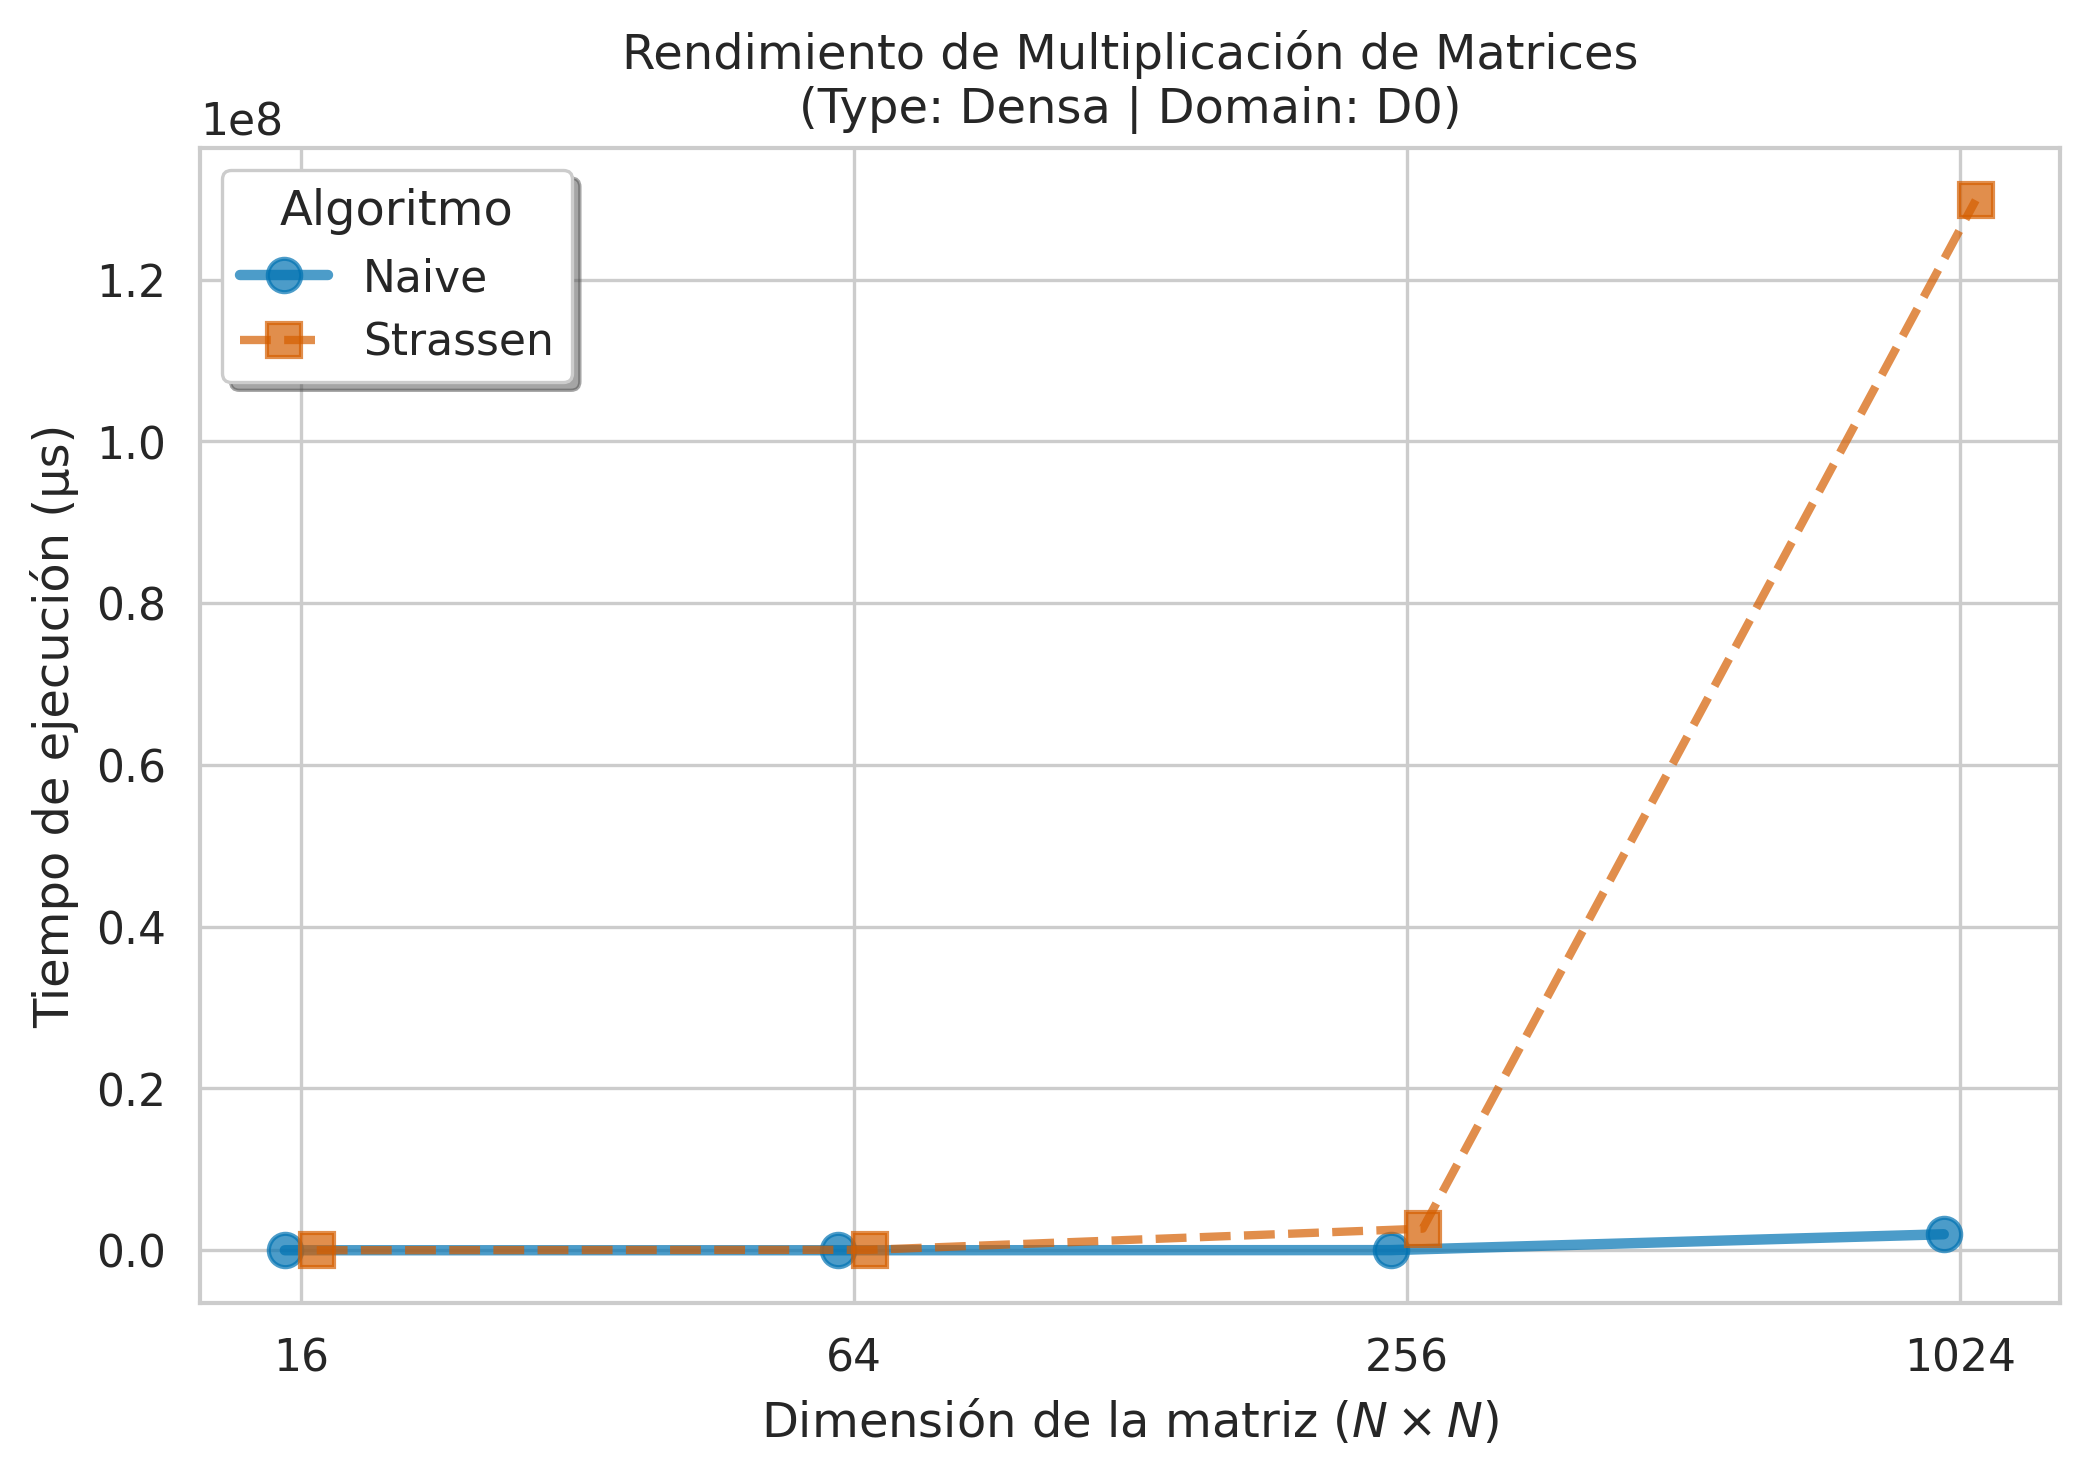
\includegraphics[width=0.7\textwidth]{../code/matrix_multiplication/data/plots/matrix_time_us_densa_D0.png}
    \caption{Tiempo de ejecución para matrices densas (Dominio D0).}
    \label{fig:matrix_densa}
\end{figure}

Al evaluar la multiplicación de matrices (Figura \ref{fig:matrix_densa} y Figura \ref{fig:matrix_memoria}) nos encontramos con una  discrepancia entre la teoría y los resultados prácticos. Teóricamente, el algoritmo de Strassen ($\mathcal{O}(N^{2.81})$) es superior al algoritmo Naive ($\mathcal{O}(N^3)$) \cite{cormen2022introduction}. Pero, en los tamaños evaluados, Naive es superior. Para el caso de matrices densas de $N=1024$, Naive finalizó en 2 segundos, mientras que Strassen llego a los 130 segundos. Esta diferencia se comprende si observamos la implementación de cada uno y cómo tratan la memoria. Naive opera mediante 3 for anidados, multiplicando y acumulando el resultado de manera directa. No requiere memoria extra durante todo el computo, esto se refleja en sus $0 KB$ de consumo adicional, posibilitando aprovechar al máximo la memoria caché. Por otro lado, Strassen para lograr una multiplicación menos, debe realizar multiples sumas y restas dividiendo el problema. Ello implica instanciar arreglos bidimensionales temporales en cada uno de los niveles recursivos. En el tamaño $N=1024$, esta creación masiva de submatrices satura el sistema operativo, provocando un consumo de memoria de $93.272 KB$. 

\begin{figure}[!htbp]
    \centering
    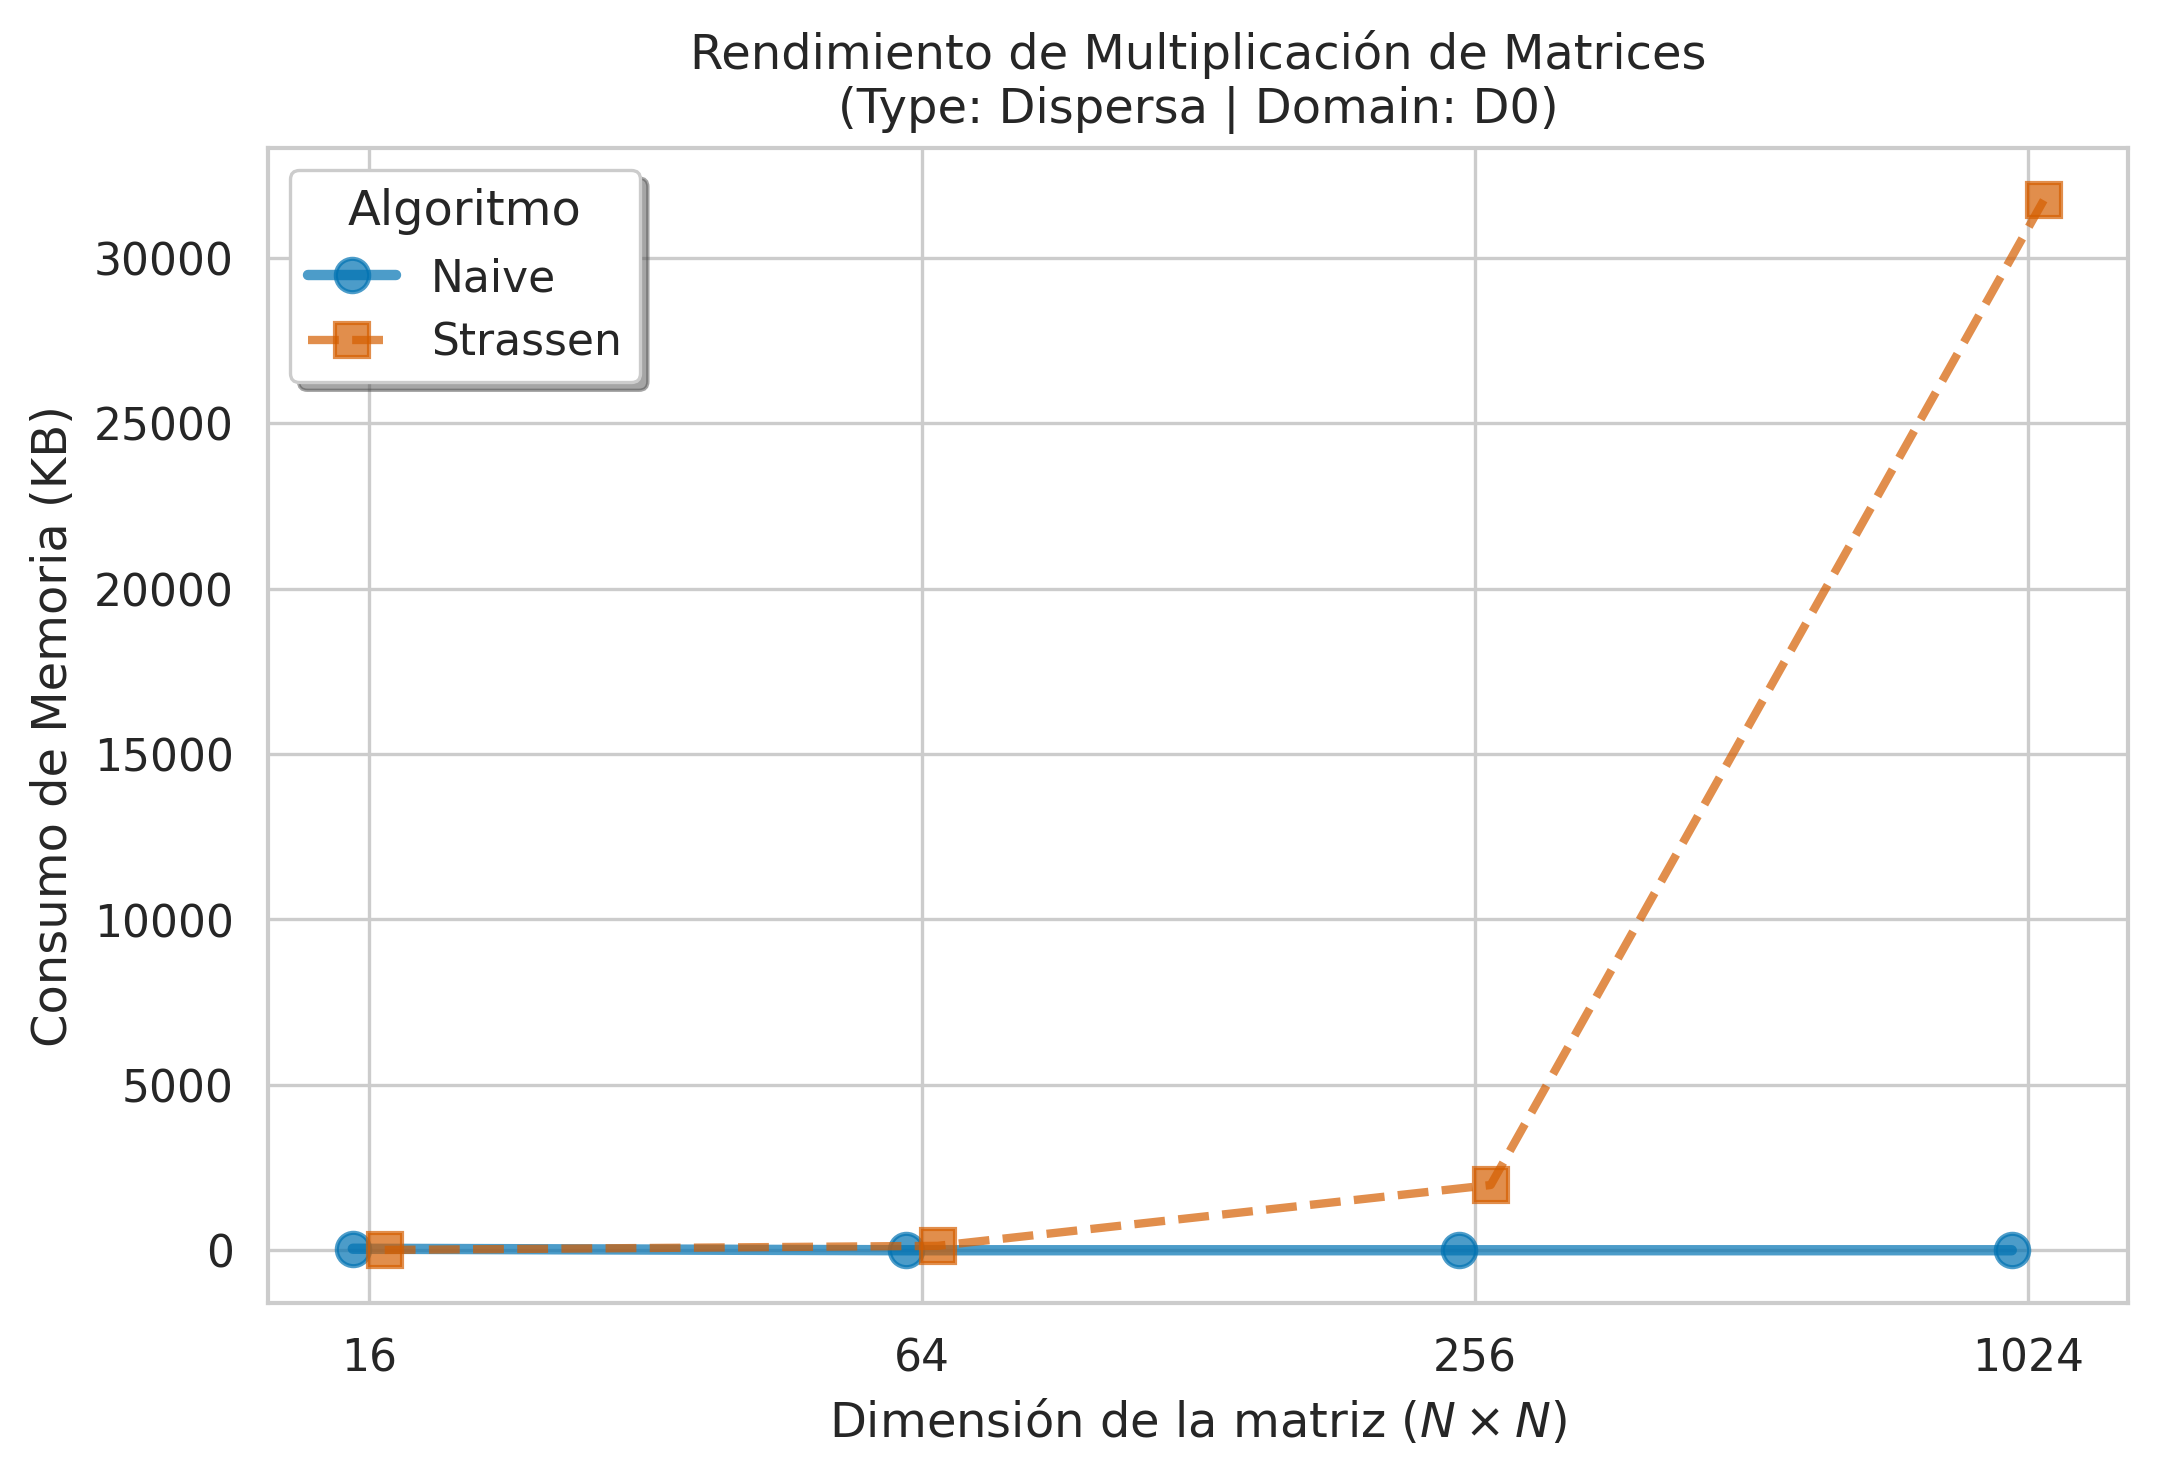
\includegraphics[width=0.7\textwidth]{../code/matrix_multiplication/data/plots/matrix_memory_kb_dispersa_D0.png}
    \caption{Consumo de memoria para matrices dispersas.}
    \label{fig:matrix_memoria}
\end{figure}

